\documentclass{beamer}
\usepackage{ctex, hyperref}
\usepackage[T1]{fontenc}

% other packages
\usepackage{latexsym,amsmath,xcolor,multicol,booktabs,calligra}
\usepackage{graphicx,pstricks,listings,stackengine}

\author{张宇驰}
\title{基于Q-学习的机器人路径规划系统}
\subtitle{结题答辩}
\institute{人工智能第10组}
\date{2021年12月16日}
\usepackage{Tsinghua}

% defs
\def\cmd#1{\texttt{\color{red}\footnotesize $\backslash$#1}}
\def\env#1{\texttt{\color{blue}\footnotesize #1}}
\definecolor{deepblue}{rgb}{0,0,0.5}
\definecolor{deepred}{rgb}{0.6,0,0}
\definecolor{deepgreen}{rgb}{0,0.5,0}
\definecolor{halfgray}{gray}{0.55}
 \lstset{ %
    language=Octave,                % the language of the code
    basicstyle=\footnotesize,           % the size of the fonts that are used for the code
    numbers=left,                   % where to put the line-numbers
    numberstyle=\tiny\color{gray},  % the style that is used for the line-numbers
    stepnumber=2,                   % the step between two line-numbers. If it's 1, each line 
                                    % will be numbered
    numbersep=5pt,                  % how far the line-numbers are from the code
    backgroundcolor=\color{white},      % choose the background color. You must add \usepackage{color}
    showspaces=false,               % show spaces adding particular underscores
    showstringspaces=false,         % underline spaces within strings
    showtabs=false,                 % show tabs within strings adding particular underscores
    frame=single,                   % adds a frame around the code
    rulecolor=\color{black},        % if not set, the frame-color may be changed on line-breaks within not-black text (e.g. commens (green here))
    tabsize=2,                      % sets default tabsize to 2 spaces
    captionpos=b,                   % sets the caption-position to bottom
    breaklines=true,                % sets automatic line breaking
    breakatwhitespace=false,        % sets if automatic breaks should only happen at whitespace
    title=\lstname,                 % show the filename of files included with \lstinputlisting;
                                    % also try caption instead of title
    keywordstyle=\color{blue},          % keyword style
    commentstyle=\color{dkgreen},       % comment style
    stringstyle=\color{mauve},         % string literal style
    escapeinside={\%*}{*)},            % if you want to add LaTeX within your code
    morekeywords={*,...}             
}


\begin{document}

\kaishu
\begin{frame}
    \titlepage
    \begin{figure}[htpb]
        \begin{center}
            
\includegraphics[width=0.2\linewidth]{pic/heu.png}
        \end{center}
    \end{figure}
\end{frame}

\begin{frame}
    \tableofcontents[sectionstyle=show,subsectionstyle=show/shaded/hide,subsubsectionstyle=show/shaded/hide]
\end{frame}


\section{课题背景}


\subsection{课题要求}

\begin{frame}{课题要求}
    

    \begin{itemize}[<+-| alert@+>] % 当然,除了alert,手动在里面插 \pause 也行
        \item 设计一个有障碍物的地图,用户可以修改障碍物布局,可以指定起点和终点
        \item 编程实现Q-学习算法,用于机器人规划最短路径,学习算法参数可以由用户设置
        \item 要求用可视化界面演示Q值变化过程及最短路径探测过程。
    \end{itemize}

\end{frame}

\begin{frame}{障碍设计}
    \item 界面初始化
    \begin{minipage}{1\linewidth}
        \medskip
        %\hspace{4cm}
        \begin{figure}[h]
            \centering
            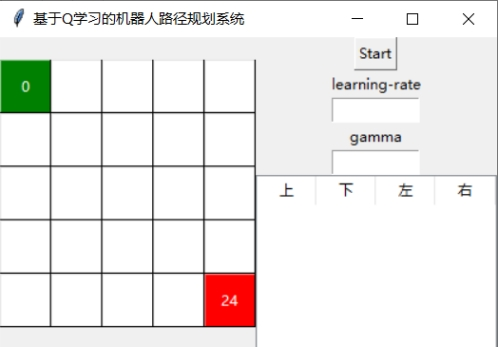
\includegraphics[height=.8\textheight]{pic/19.jpg}
        \end{figure}
    \end{minipage}
\end{frame}

\begin{frame}{障碍设计}
    \item 界面初始化参数及障碍物设置
    \begin{minipage}{1\linewidth}
        \medskip
        %\hspace{4cm}
        \begin{figure}[h]
            \centering
            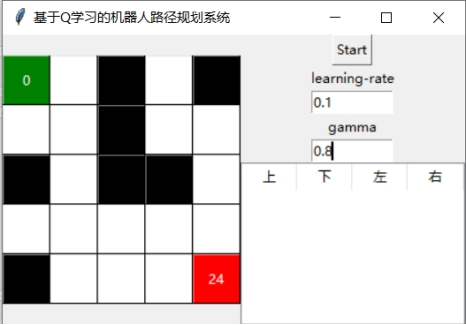
\includegraphics[height=.8\textheight]{pic/20.jpg}
        \end{figure}
    \end{minipage}
\end{frame}

\begin{frame}{障碍设计}
    \item 程序运行
    \begin{minipage}{1\linewidth}
        \medskip
        %\hspace{4cm}
        \begin{figure}[h]
            \centering
            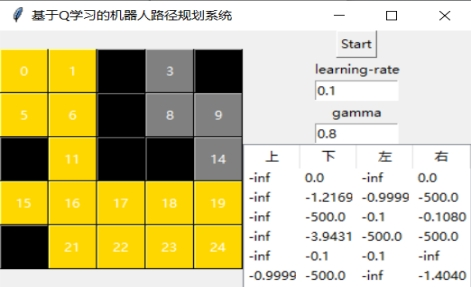
\includegraphics[height=.8\textheight]{pic/21.jpg}
        \end{figure}
    \end{minipage}
\end{frame}


\begin{frame}{最终地图}

    
    \begin{minipage}{1\linewidth}
        \medskip
        %\hspace{4cm}
        \begin{figure}[h]
            \centering
            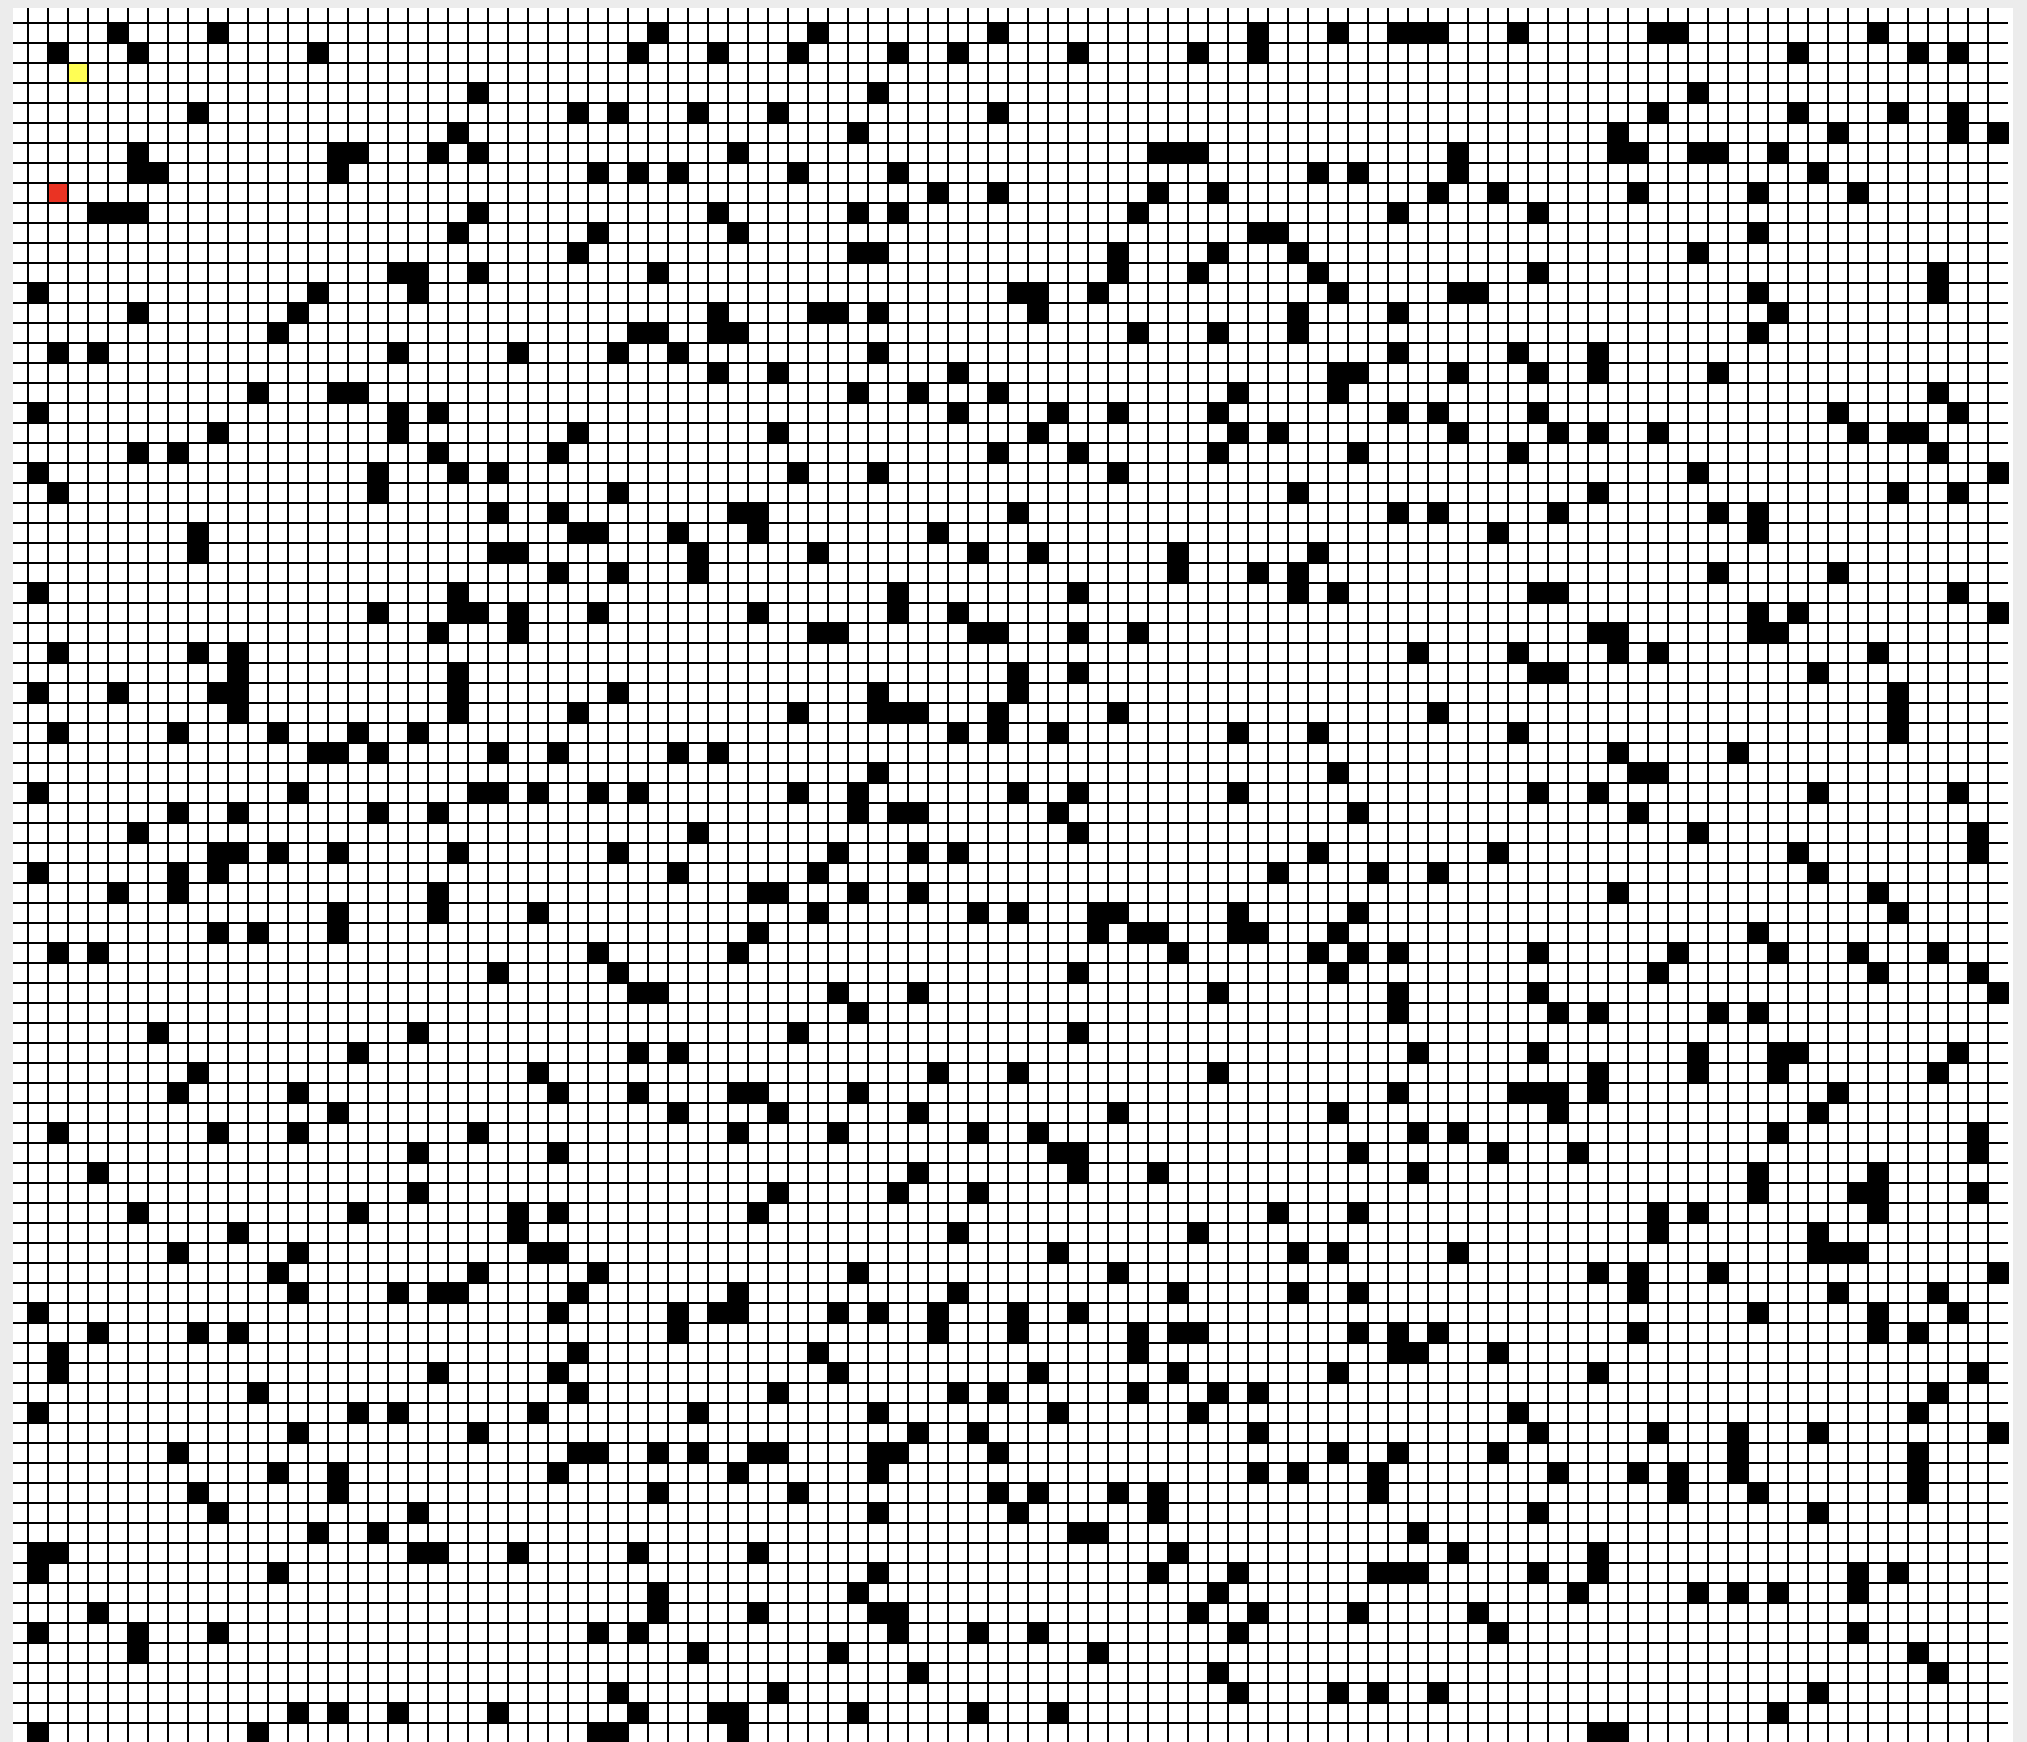
\includegraphics[height=.8\textheight]{pic/2.png}
        \end{figure}
    \end{minipage}
\end{frame}


\subsection{小组分工}
\begin{frame}{小组分工}
    \begin{itemize}
        \tiny
        \item 张宇驰(2019201426):封装地图、q\_learning相关函数,主函数设计及代码连接
        \item 王瑞晗(2019041517):分析题干要求,分析Q-学习的路径规划算法,对用户界面的设计及代码实现,数据归纳
        \item 赵  轩(2019201428):设计地图中处理边界代码,调整训练参数以达到更好的效果
        \item 李皓雯(2019065109):可视化界面中Q表表格的设计,调试bug
        \item 许德彬(2019201425):可视化界面中开始按钮、输入输出的设计,调式bug
    \end{itemize}
\end{frame}



\section{Q-learning算法}
\begin{frame}{简介}

    \begin{itemize}[<+-| alert@+>]
        
        
        \item 强化学习作为机器学习算法的一种,其模式是让智能体在“训练”中学到“经验”,以实现给定的任务。
        
        \item QLearning属于时序差分学习。该算法结合了动态规划和蒙特卡罗MC算法,模拟(或者经历)一个情节,每行动一步(或多步)后,根据新状态的价值,来估计执行前的状态价值。以此来达到学习目的
    \end{itemize}
\end{frame}

\subsection{行为准则}

\begin{frame}{对于我们的路径规划问题}
    \begin{itemize}
         
        
        \item 每个坐标代表一个状态,每个状态下有四个可选择的动作(向上向下向左向右)
        
        \item 执行不同动作会到达一个新的状态(即坐标),此时会获得一个reward值,表示我们根据经验“将会”获得的奖励
        
        \item 这里的“将会”其实是一种估计,随着不断地学习完善,经验会越来越丰富,这里的奖励值也可能会改变
        
        \item 我们进行的q\_learning实际就是不断完善经验完善这个reward奖励机制的过程
    \end{itemize}
\end{frame}


\subsection{Q\_Learning 决策}
\begin{frame}{Q\_Learning 决策}
    \begin{itemize}[<+-| alert@+>]
        \tiny
        \begin{minipage}{0.5\linewidth}
            \medskip
            %\hspace{2cm}
            \begin{figure}[h]
                \centering
                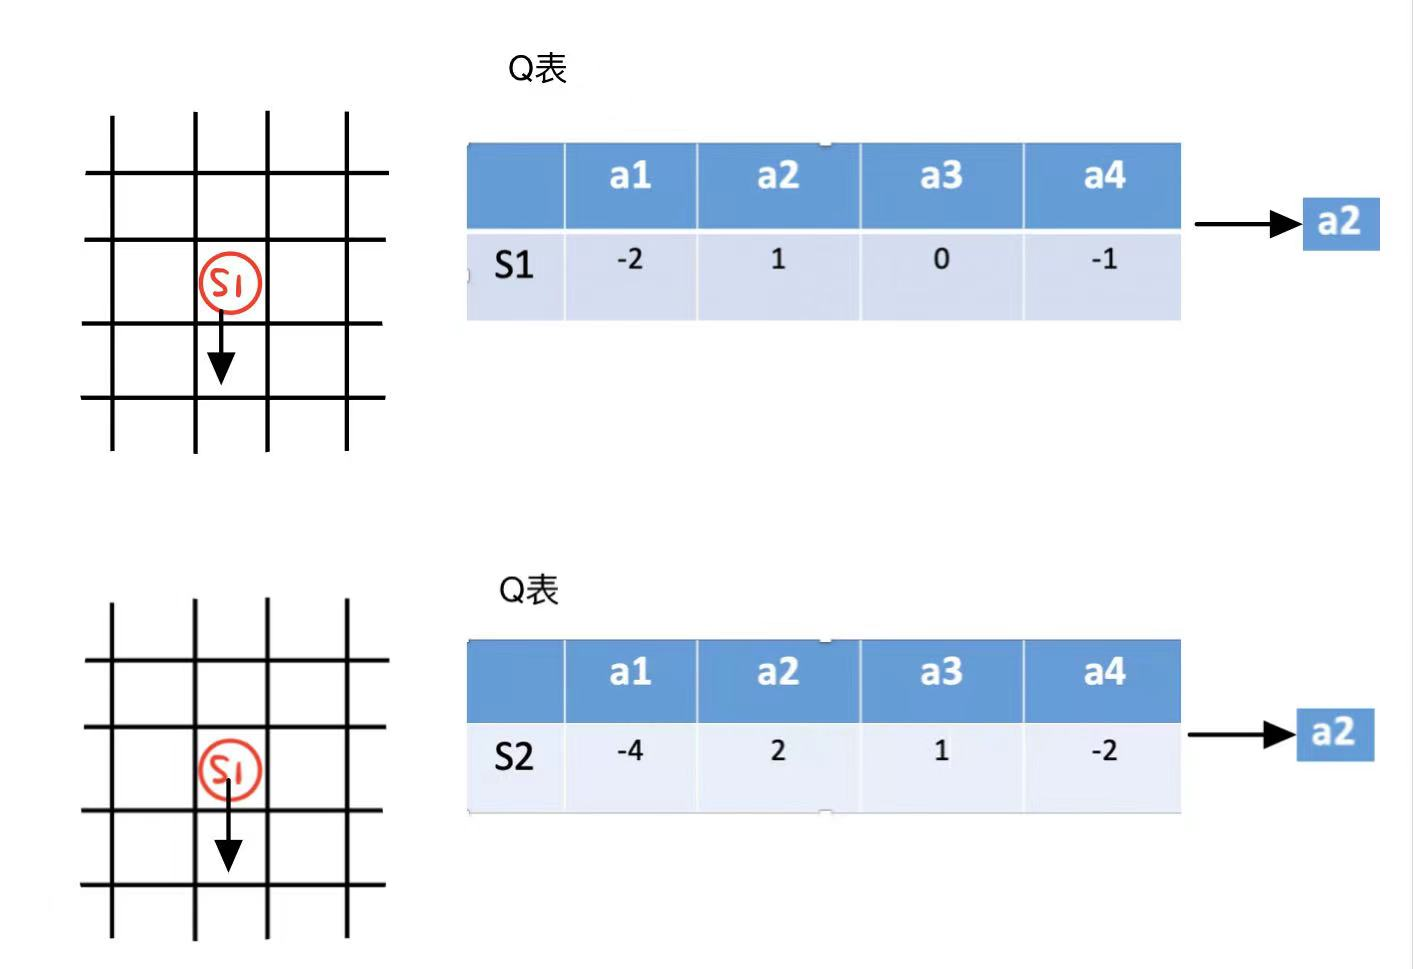
\includegraphics[height=.4\textheight]{pic/4.jpg}
            \end{figure}
        \end{minipage}
        
        \item 假设我们的行为准则已经学习好了,现在我们处于状态 $s_1$ ,          假设在 $( x_0 , y_0 )$ 点. 
        
        
        \item 我们有四个行为$a_1,a_2,a_3,a_4$分别是向上走,向下走, 向左走 ,向上走.
        根据我们的经验,假设在这种$s_1$状态下,$a_2$向下走带来的潜在奖励要比其余动作高。这里的潜在奖励我们可以用一个有关于s和a的Q表格代替,在我的记忆Q表格中, $Q(s_1, a_2)$要大于 $Q(s_1, a_1)$ , $Q(s_1, a_1) , Q(s_1, a_3) , Q(s_1, a_4),$ 所以我们判断要选择 $a_2$ 作为下一个行为. 
        
        \item 现在我们的状态更新成 $s_2 $, 我们还是有四个同样的选择, 重复上面的过程, 在行为准则Q 表中寻找s2状态下$Q(s_2, a_i)$最大的值.
        
        \item 接着根据 $a_2 $我们到达$ s_3 $并在此重复上面的决策过程. 
        Q\_learning 的方法也就是这样决策的. 
    \end{itemize}
\end{frame}

\subsection{Q\_Learning 更新}
\begin{frame}{Q\_Learning 更新}
    \begin{itemize}
        \tiny
        \begin{minipage}{0.5\linewidth}
            \medskip
            %\hspace{2cm}
            \begin{figure}[h]
                \centering
                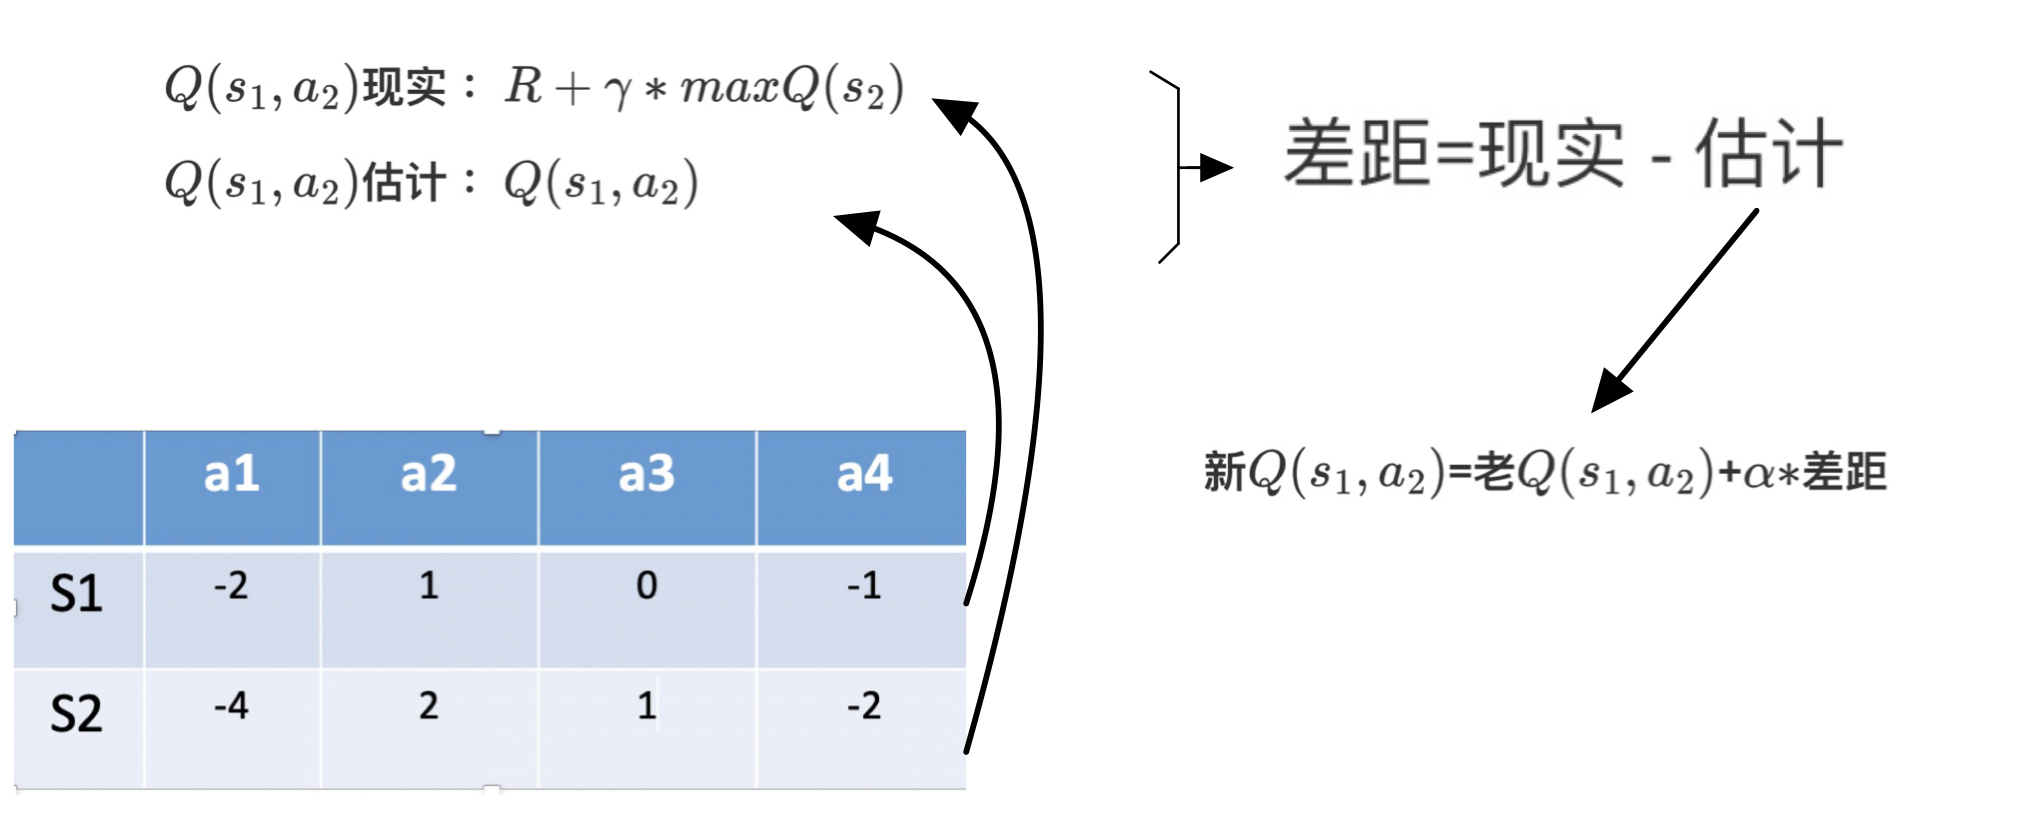
\includegraphics[height=.4\textheight]{pic/5.jpg}
            \end{figure}
        \end{minipage}
        \item 我们回到之前的流程, 根据 Q 表的估计, 因为在 $s_1$ 中, $a_2$ 的值比较大, 通过之前的决策方法, 我们在 $s_1$ 采取了 a2, 并到达 $s_2$, 这时我们开始更新用于决策的 Q 表, 接着我们并没有在实际中采取任何行为, 而是再想象自己在 $s_2$ 上采取了每种行为, 分别看看两种行为哪一个的 Q 值大, 我们把大的 $Q(s_2, a_2)$ 乘上一个衰减值 gamma (比如是0.9) 并加上到达$s_2$时所获取的奖励 R , 因为会获取实实在在的奖励 R , 我们将这个作为我现实中 $Q(s_1, a_2)$ 的值, 但是我们之前是根据 Q 表估计 $Q(s_1, a_2)$ 的值. 所以有了现实和估计值, 我们就能更新$Q(s_1, a_2)$ , 根据 估计与现实的差距, 将这个差距乘以一个学习效率 alpha 累加上老的 $Q(s_1, a_2)$的值 变成新的值. 但时刻记住, 我们虽然用 $maxQ(s_2)$ 估算了一下 $s_2$ 状态, 但还没有在 $s_2$ 做出任何的行为, $s_2$ 的行为决策要等到更新完了以后再重新另外做. 这就是 off-policy 的 Q learning 是如何决策和学习优化决策的过程.
    \end{itemize}
\end{frame}

\subsection{Q\_Learning 整体算法}
\begin{frame}
    \begin{minipage}{0.5\linewidth}
        \medskip
        %\hspace{2cm}
        \begin{figure}[h]
            \centering
            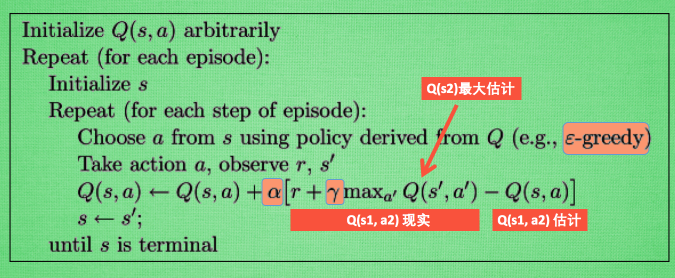
\includegraphics[height=.4\textheight]{pic/3.png}
        \end{figure}
    \end{minipage}
    \tiny
    \item 这一张图概括了我们之前所有的内容. 这也是 Q learning 的算法, 每次更新我们都用到了 Q 现实和 Q 估计, 而且 Q learning 的迷人之处就是 在 Q(s1, a2) 现实 中, 也包含了一个 Q(s2) 的最大估计值, 将对下一步的衰减的最大估计和当前所得到的奖励当成这一步的现实, 很奇妙吧. 最后我们来说说这套算法中一些参数的意义. Epsilon greedy 是用在决策上的一种策略, 比如 epsilon = 0.9 时, 就说明有90\% 的情况我会按照 Q 表的最优值选择行为, 10\% 的时间使用随机选行为. alpha是学习率, 来决定这次的误差有多少是要被学习的, alpha是一个小于1 的数. gamma 是对未来 reward 的衰减值. 我们可以这样想象.
    
\end{frame}


\subsection{Q\_Learning 中的 Gamma}
\begin{frame}
    \begin{itemize}
        \tiny
        \begin{minipage}{0.5\linewidth}
        \medskip
        %\hspace{2cm}
        \begin{figure}[h]
            \centering
            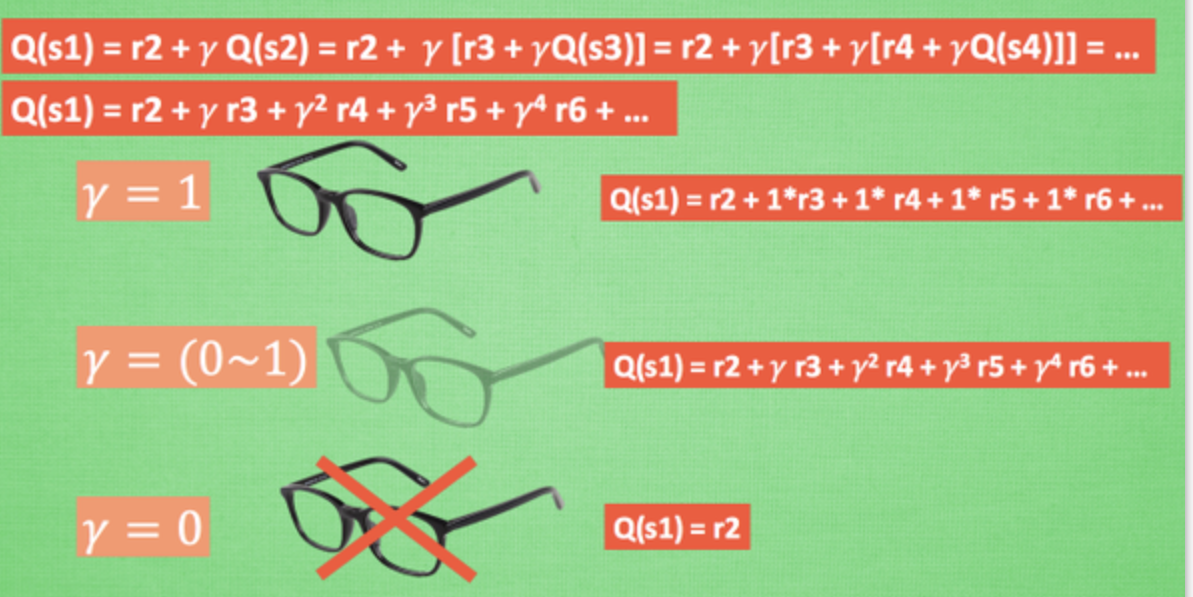
\includegraphics[height=.4\textheight]{pic/22.png}
        \end{figure}
    \end{minipage}
        \item 我们重写一下 Q(s1) 的公式, 将 Q(s2) 拆开, 因为Q(s2)可以像 Q(s1)一样,是关于Q(s3) 的, 所以可以写成这样, 然后以此类推, 不停地这样写下去, 最后就能写成这样, 可以看出Q(s1) 是有关于之后所有的奖励, 但这些奖励正在衰减, 离 s1 越远的状态衰减越严重. 不好理解? 行, 我们想象 Qlearning 的机器人天生近视眼, gamma = 1 时, 机器人有了一副合适的眼镜, 在 s1 看到的 Q 是未来没有任何衰变的奖励, 也就是机器人能清清楚楚地看到之后所有步的全部价值, 但是当 gamma =0, 近视机器人没了眼镜, 只能摸到眼前的 reward, 同样也就只在乎最近的大奖励, 如果 gamma 从 0 变到 1, 眼镜的度数由浅变深, 对远处的价值看得越清楚, 所以机器人渐渐变得有远见, 不仅仅只看眼前的利益, 也为自己的未来着想.
    \end{itemize}
\end{frame}

\section{地图环境}
\subsection{代码主结构}

\begin{frame}{代码主结构}
    \begin{itemize}
    \tiny
    \item 
    \begin{minipage}{1\linewidth}
        \medskip
        %\hspace{4cm}
        \begin{figure}[h]
            \centering
            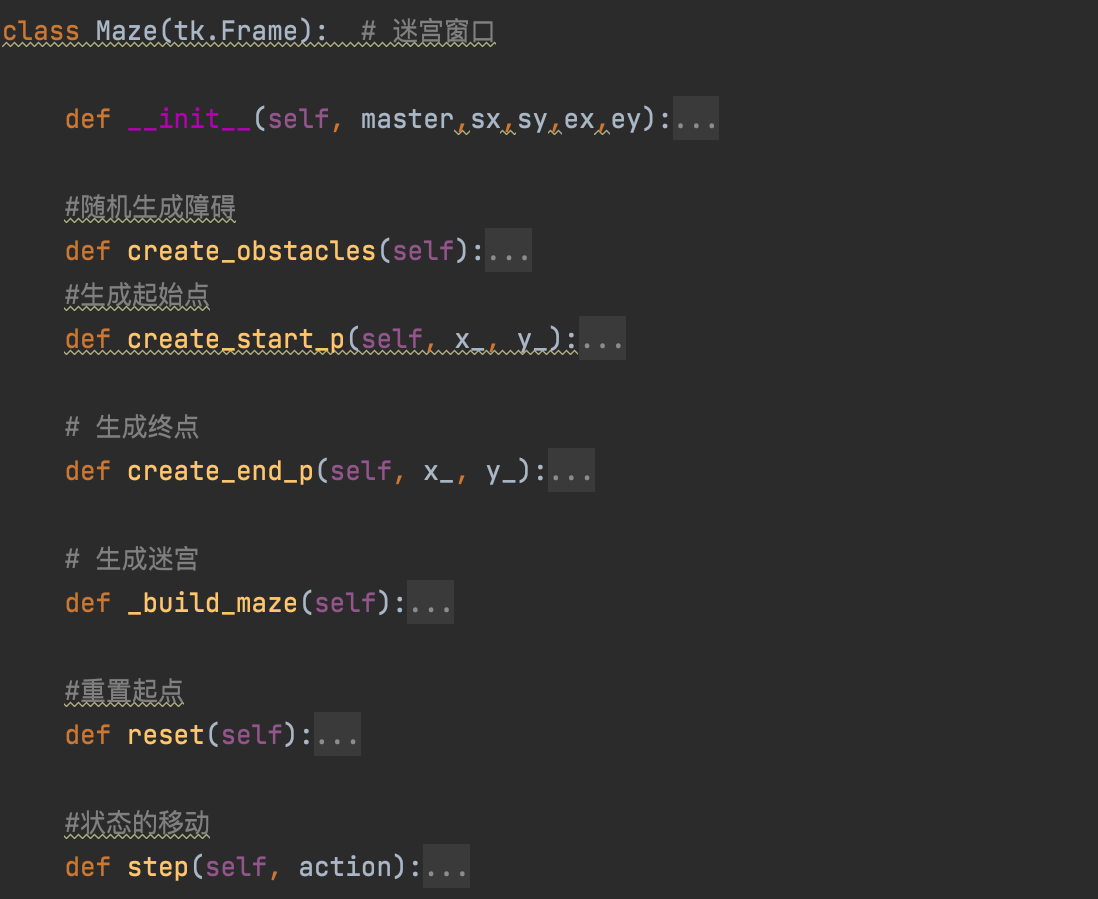
\includegraphics[height=.8\textheight]{pic/11.png}
        \end{figure}
    \end{minipage}
    \end{itemize}
\end{frame}


\subsection{预设值}

\begin{frame}{预设值}
    \begin{itemize}
    \item 
    \\
    \\
    \\
    \begin{minipage}{1\linewidth}
        \medskip
        %\hspace{4cm}
        \begin{figure}[h]
            \centering
            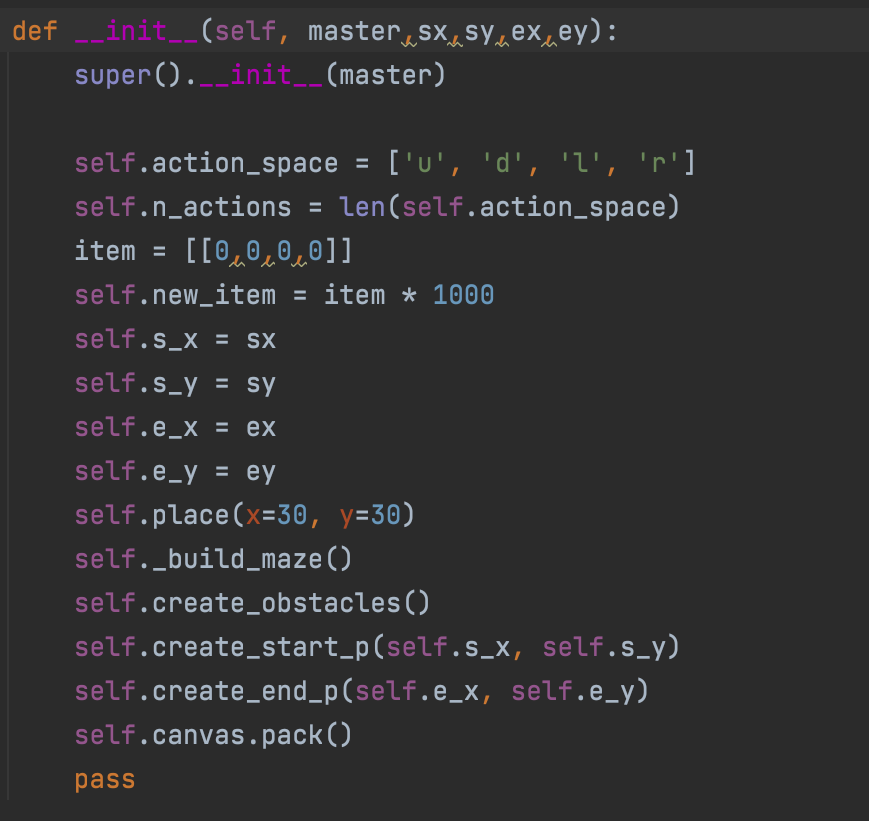
\includegraphics[height=.8\textheight]{pic/12.png}
        \end{figure}
    \end{minipage}
    
    \end{itemize}
    
\end{frame}


\subsection{生成障碍、起始点}

\begin{frame}{生成障碍、起始点}
    \begin{itemize}
    \tiny
        \item 
        \begin{minipage}{1\linewidth}
        \medskip
        %\hspace{4cm}
        \begin{figure}[h]
            \centering
            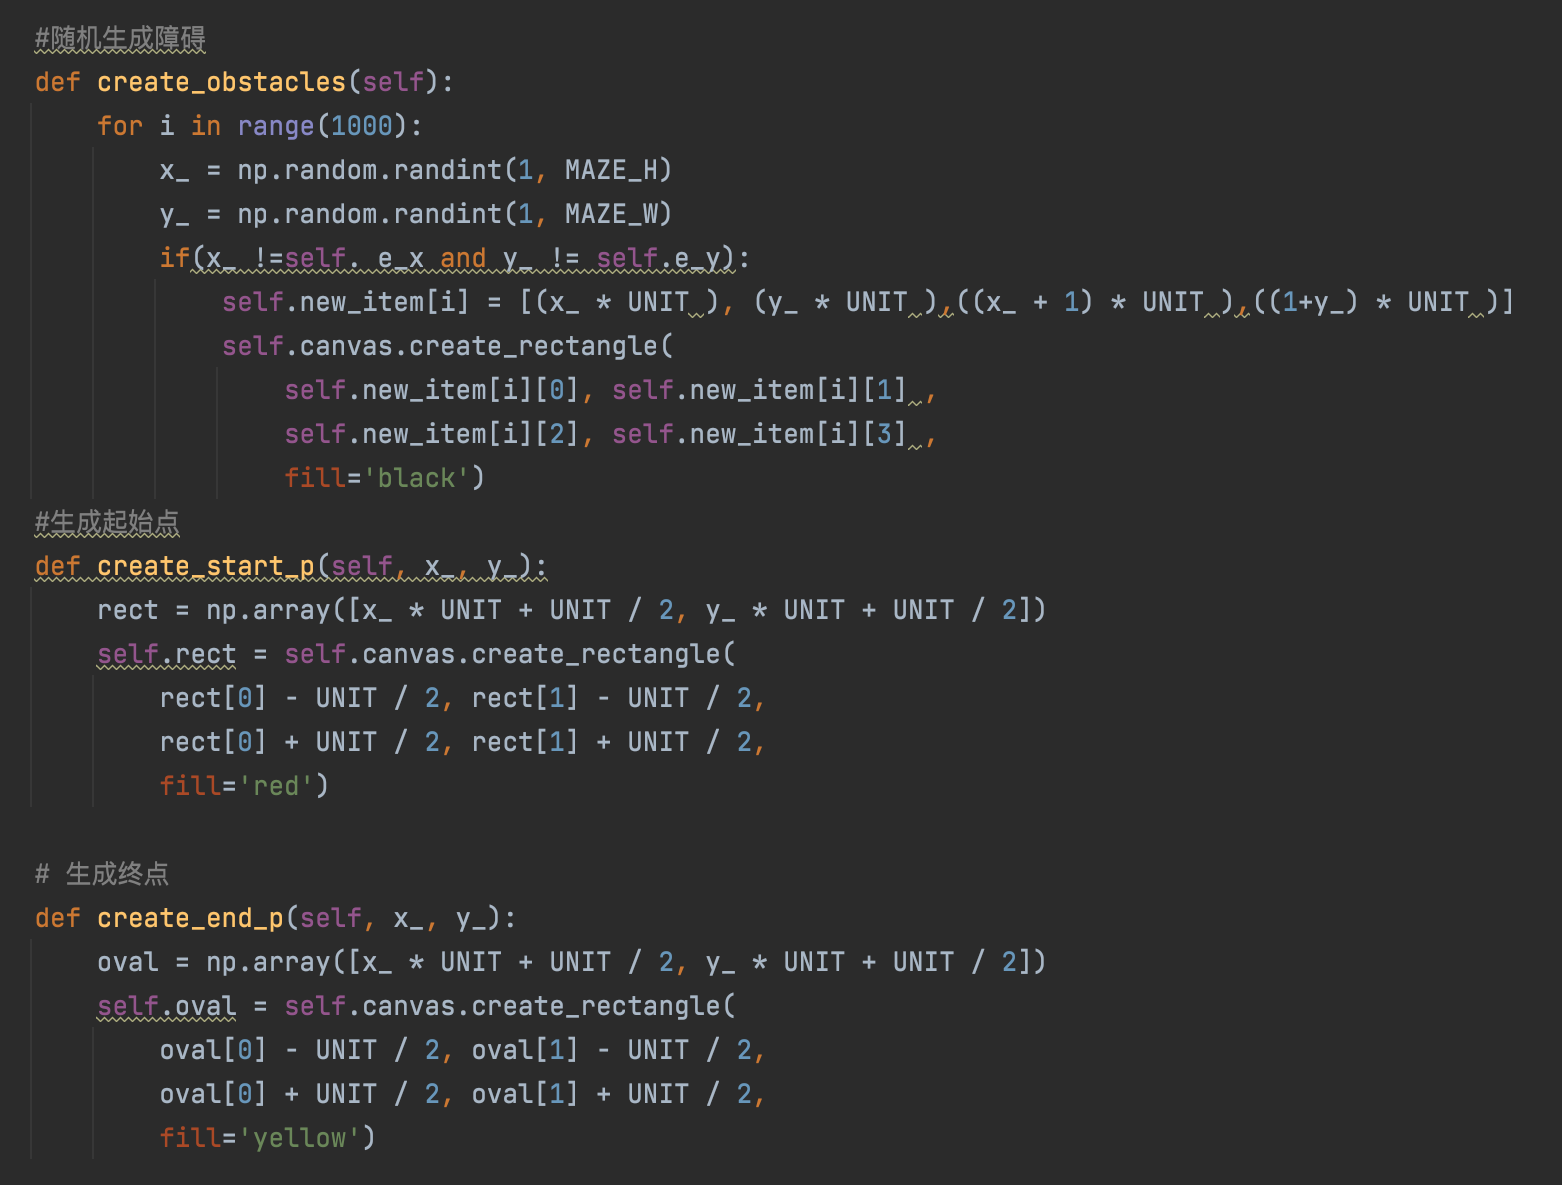
\includegraphics[height=.8\textheight]{pic/13.png}
        \end{figure}
    \end{minipage}
    \end{itemize}
\end{frame}

\subsection{地图刷新 }
\begin{frame}{地图刷新}
    \begin{itemize}
    \tiny
    \item 
    
        \begin{minipage}{1\linewidth}
        \medskip
        %\hspace{4cm}
        \begin{figure}[h]
            \centering
            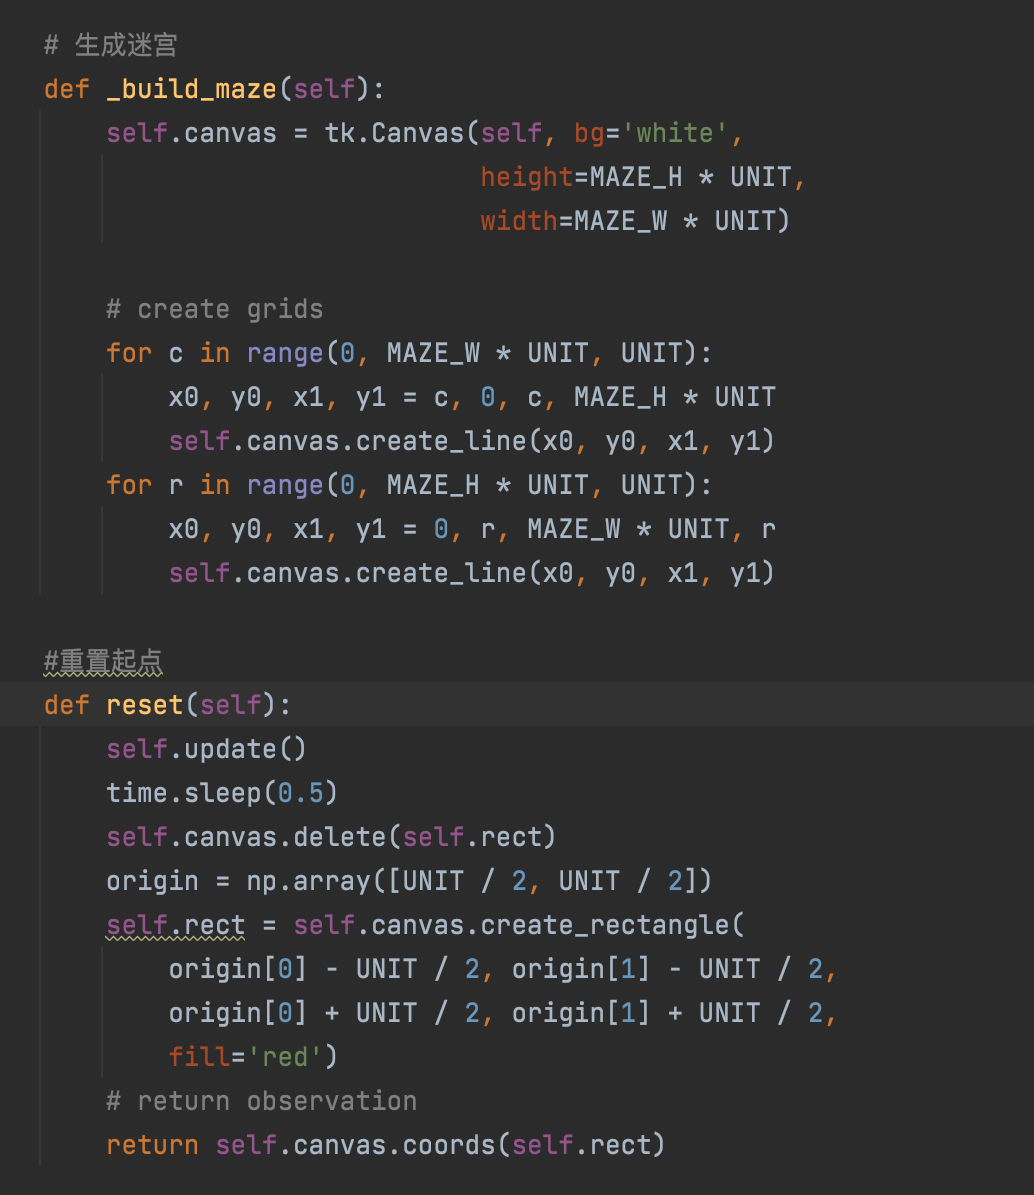
\includegraphics[height=.8\textheight]{pic/14.png}
        \end{figure}
    \end{minipage}
    
    \end{itemize}
    
\end{frame}


\subsection{状态的移动 }
\begin{frame}{状态的移动}
    \begin{itemize}
    \tiny
    
    \item 
    \\
    
    \begin{minipage}{1\linewidth}
        \medskip
        %\hspace{4cm}
        \begin{figure}[h]
            \centering
            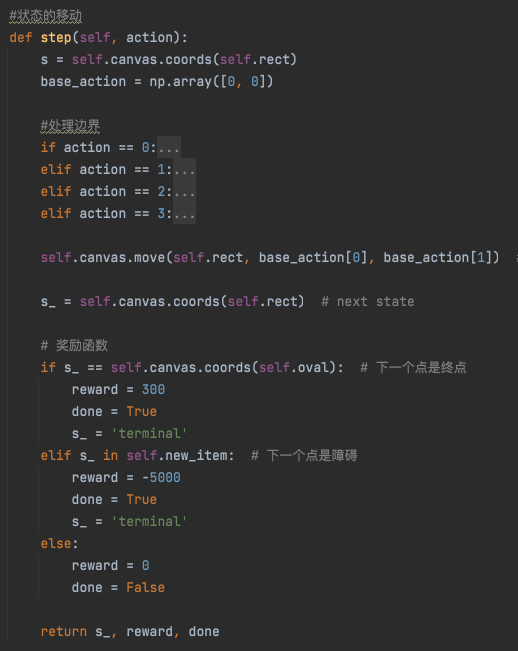
\includegraphics[height=.8\textheight]{pic/15.png}
        \end{figure}
    \end{minipage}
    \end{itemize}
    
\end{frame}



\section{思维决策}
\subsection{代码主结构}

\begin{frame}{代码主结构}
    \begin{itemize}
    \tiny
    \item 我们将要以一个 class 形式定义 Q learning, 并把这种 tabular q learning 方法叫做 QLearningTable.
    \begin{minipage}{0.5\linewidth}
        \medskip
        %\hspace{2cm}
        \begin{figure}[h]
            \centering
            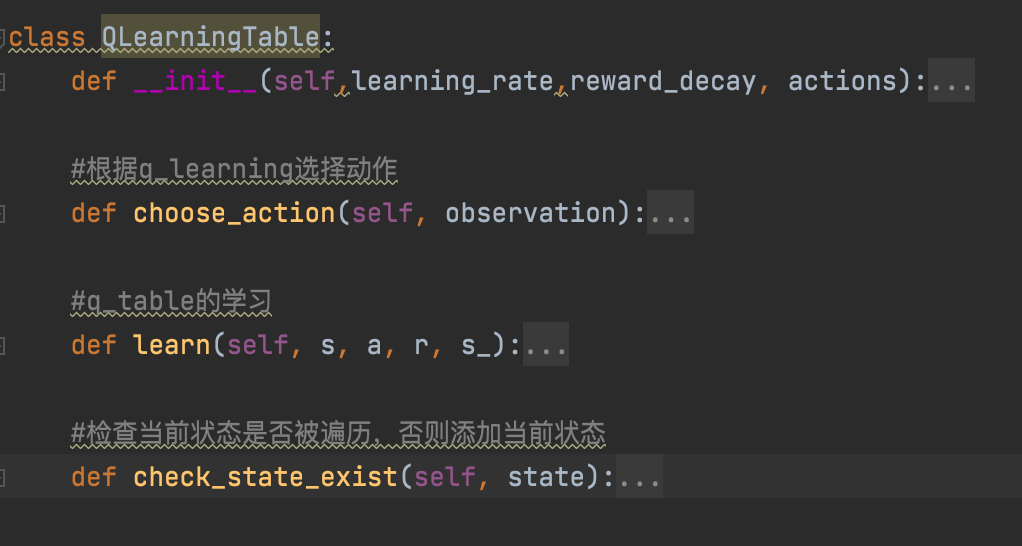
\includegraphics[height=.4\textheight]{pic/6.png}
        \end{figure}
    \end{minipage}
    \end{itemize}
\end{frame}


\subsection{预设值}

\begin{frame}{预设值}
    \begin{itemize}
    \item 需要的模块和参数设置:
    \\
    \begin{minipage}{0.5\linewidth}
        \medskip
        %\hspace{2cm}
        \begin{figure}[h]
            \centering
            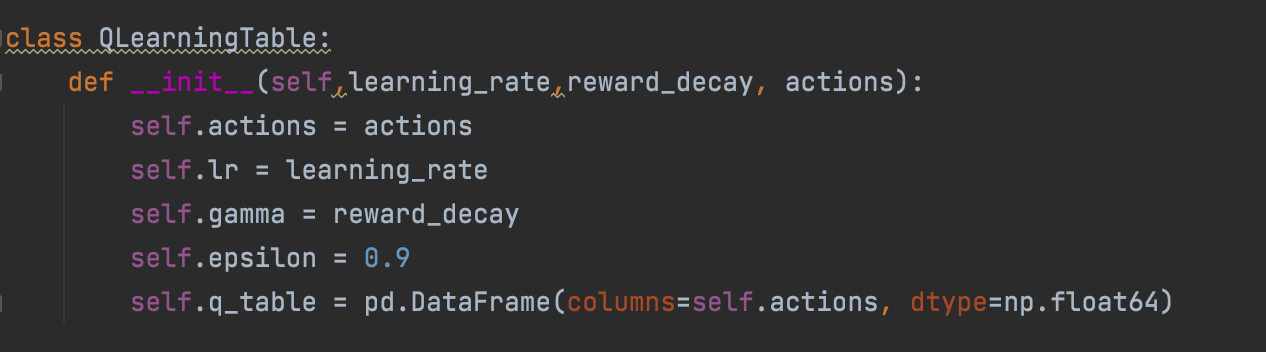
\includegraphics[height=.4\textheight]{pic/7.png}
        \end{figure}
    \end{minipage}
    
    \end{itemize}
    
\end{frame}


\subsection{决定行为}

\begin{frame}{决定行为}
    \begin{itemize}
    \tiny
        \item 这里是定义如何根据所在的 state, 或者是在这个 state 上的 观测值 (observation) 来决策.
        \begin{minipage}{0.5\linewidth}
        \medskip
        %\hspace{2cm}
        \begin{figure}[h]
            \centering
            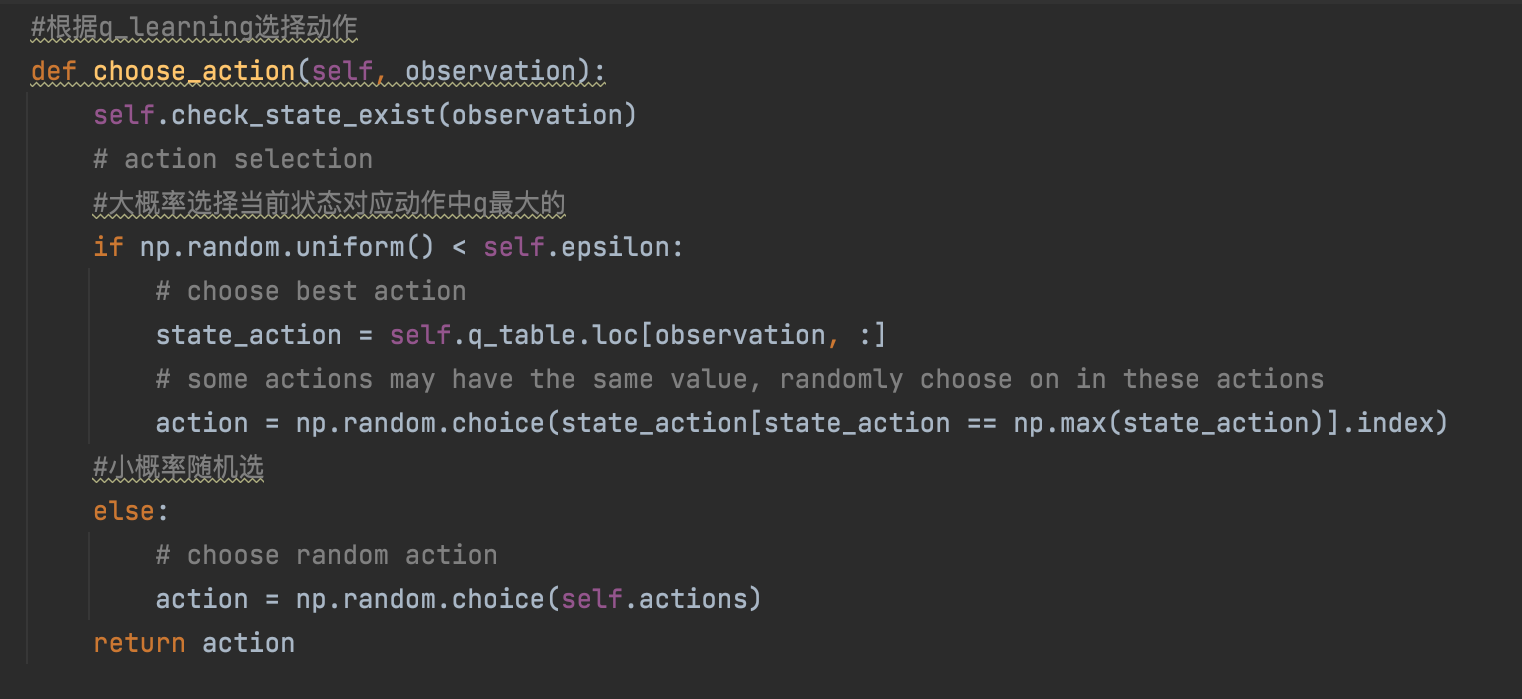
\includegraphics[height=.4\textheight]{pic/8.png}
        \end{figure}
    \end{minipage}
    \end{itemize}
\end{frame}

\subsection{学习 }
\begin{frame}{学习}
    \begin{itemize}
    \tiny
    \item 我们根据是否是 terminal state (回合终止符) 来判断应该如何更行 q\_table. 
    这可以理解成神经网络中的更新方式, 学习率 * (真实值 - 预测值). 将判断误差传递回去, 有着和神经网络更新的异曲同工之处.
    
        \begin{minipage}{0.5\linewidth}
        \medskip
        %\hspace{2cm}
        \begin{figure}[h]
            \centering
            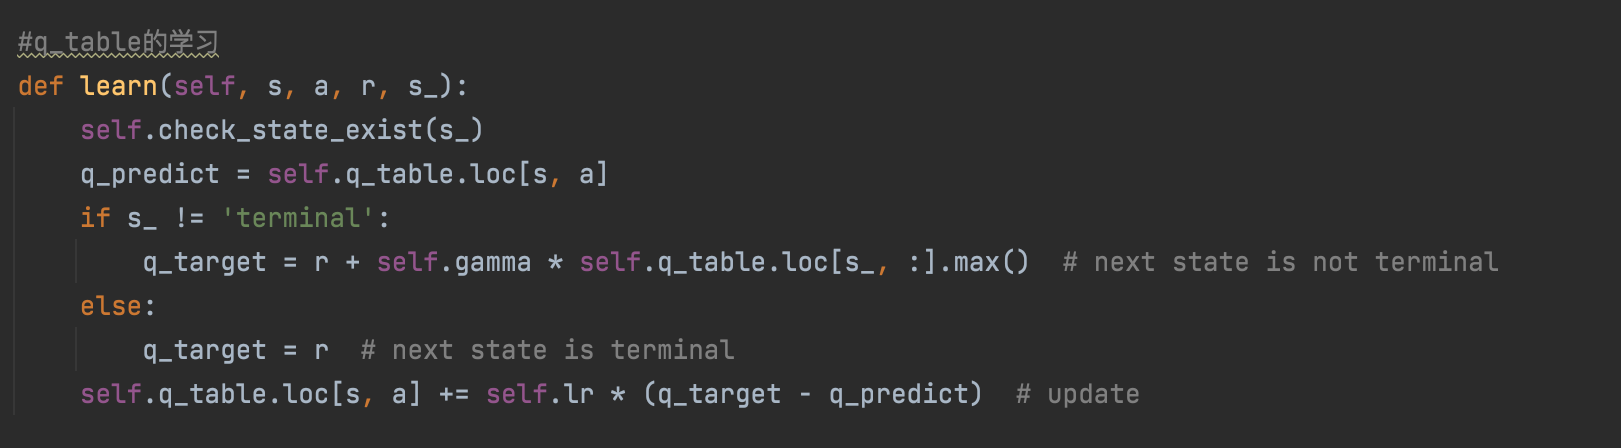
\includegraphics[height=.4\textheight]{pic/9.png}
        \end{figure}
    \end{minipage}
    
    \end{itemize}
    
\end{frame}


\subsection{检测 state 是否存在 }
\begin{frame}{检测 state 是否存在}
    \begin{itemize}
    \tiny
    
    \item 这个功能就是检测 q\_table 中有没有当前 state 的步骤了, 如果还没有当前 state, 那我我们就插入一组全 0 数据, 当做这个 state 的所有 action 初始 values.
    \\
    
    \begin{minipage}{0.5\linewidth}
        \medskip
        %\hspace{2cm}
        \begin{figure}[h]
            \centering
            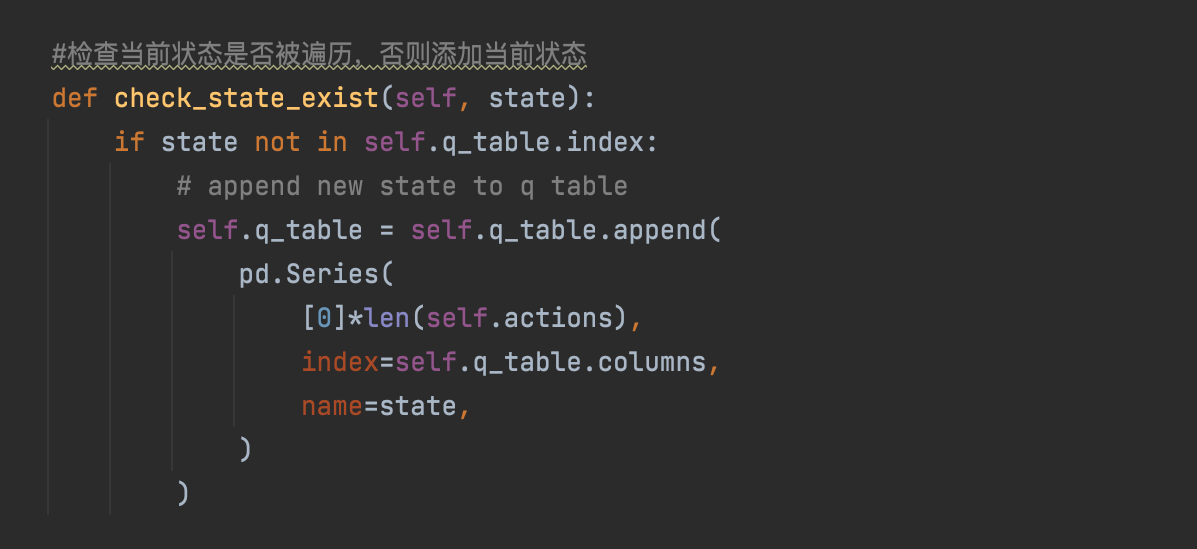
\includegraphics[height=.4\textheight]{pic/10.png}
        \end{figure}
    \end{minipage}
    \end{itemize}
\end{frame}

\section{主函数}
\begin{frame}{主函数}
    \begin{itemize}
    \tiny
    
    \item 
    \\
    
    \begin{minipage}{1\linewidth}
        \medskip
        %\hspace{4cm}
        \begin{figure}[h]
            \centering
            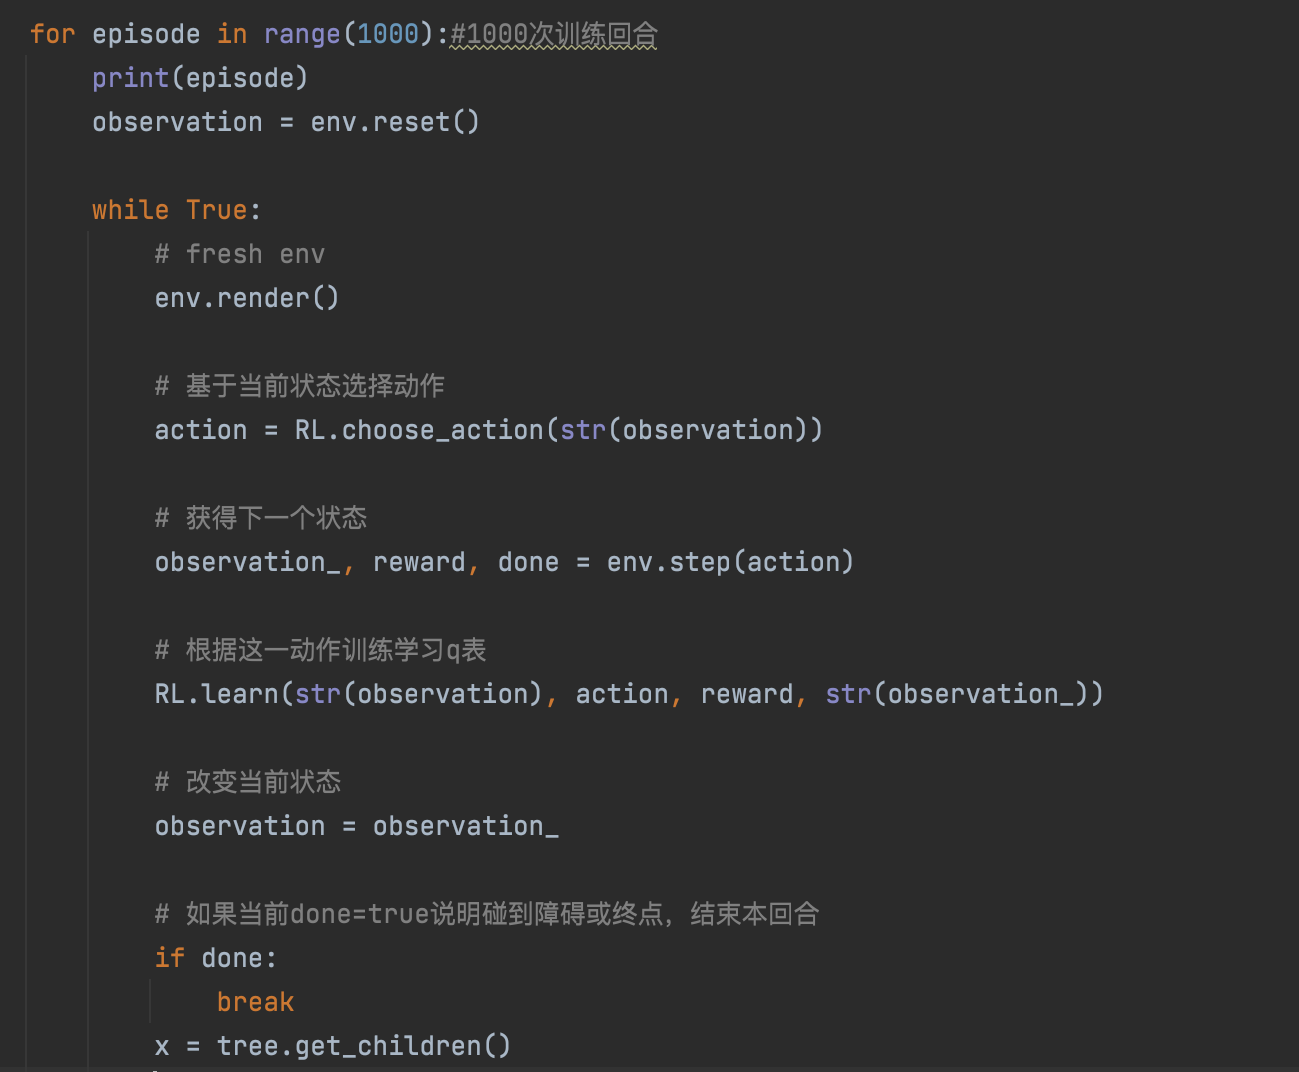
\includegraphics[height=.8\textheight]{pic/16.png}
        \end{figure}
    \end{minipage}
    \end{itemize}
    
\end{frame}

\section{运行演示}



\section{数据归纳}
\begin{frame}{数据归纳}
    \begin{itemize}
    \tiny
    \item 经多次实验统计,我们得知该学习在对应轮次下的探索优化度大致如下:
    
    
        \begin{minipage}{0.5\linewidth}
        \medskip
        %\hspace{2cm}
        \begin{figure}[h]
            \centering
            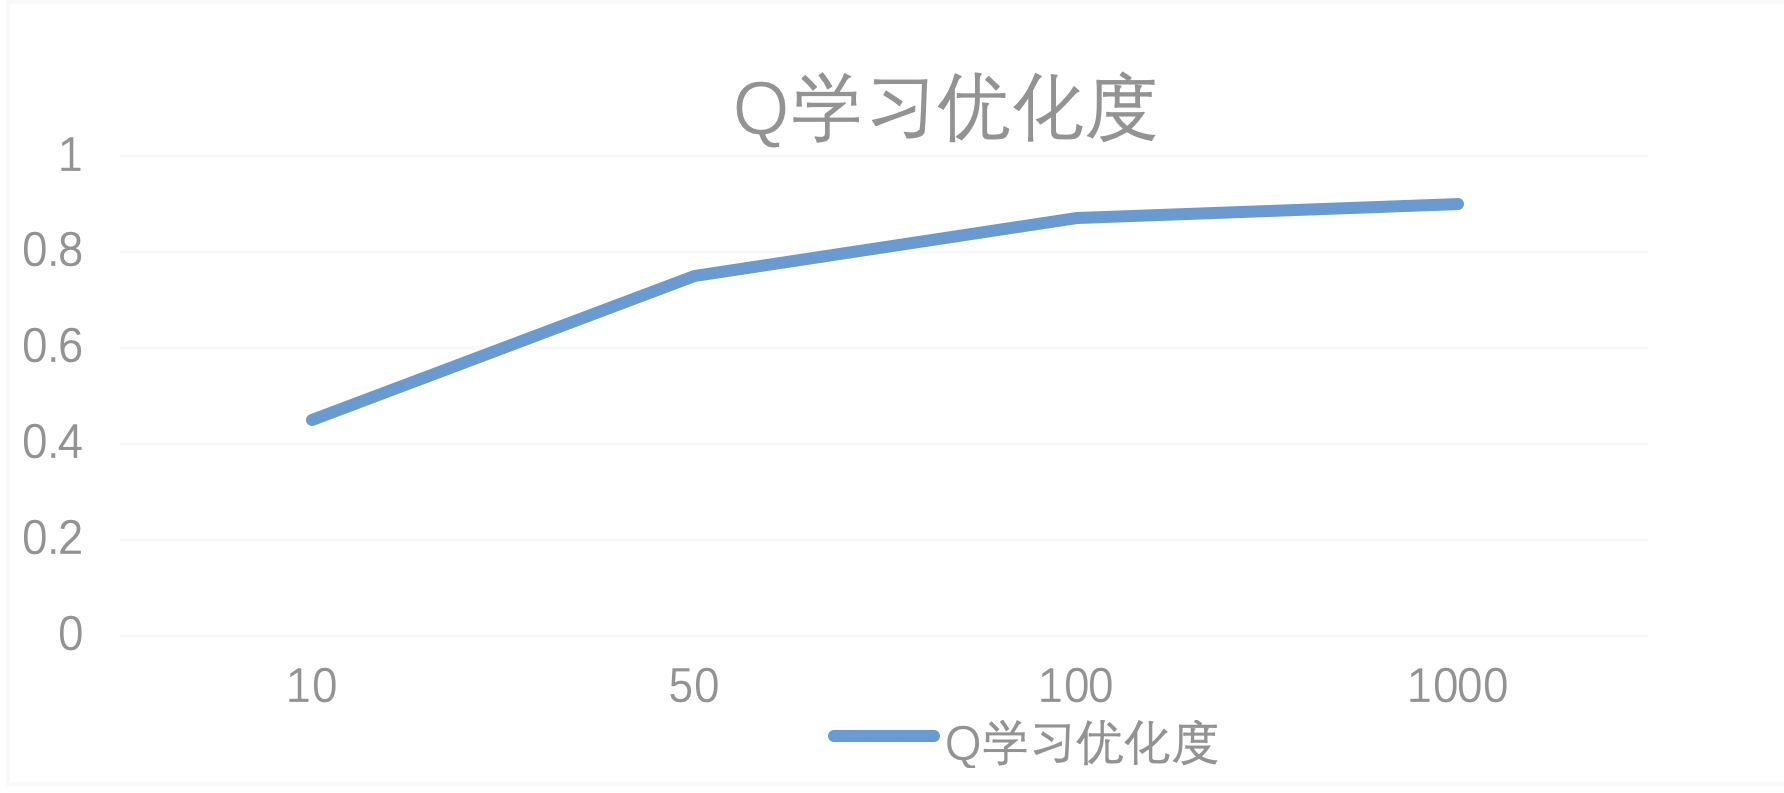
\includegraphics[height=.4\textheight]{pic/17.png}
        \end{figure}
    \end{minipage}
    
    \item 可见,该曲线在初始100次训练时增长率交高,随后放缓,并且无限趋近于0.9,这是因为,设置的epsilon为0.9的缘故,无论Q学习的精度多高,都有10\%的概率会进行随机探索。
    
    \end{itemize}
    
\end{frame}


\begin{frame}{强化学习中性能的评价指标到底应该如何选择?}
    \begin{itemize}
    \tiny
    \item 据了解,性能评价指标大致存在两种:1.平均得分法2.平均Q值法
    \item 平均得分。测试性能时agent进行一定的步数执行,记录agent所获得的所有奖励值并对其求平均。
    \item 平均Q值。测试性能前就确定好一定数量的状态动作对,测试时对已经确定好的状态动作对的Q值求平均。
    \item 平均得分法的评价方法:不同episode下对应的得分随episode数(training epochs数)变化会具备较大的抖动性,相邻episode(training epochs)对应的得分往往有很大差距,但是从整体来看平均得分法依然可以看到整体性能的变化趋势。
    \item 平均Q值的方法,可以看到不同episode(training epochs)对应的Q值变化趋势比较平稳。
   \end{itemize}
    
\end{frame}

\begin{frame}{强化学习中性能的评价指标到底应该如何选择?}
    \begin{itemize}
    \tiny
    \item 图1.2使用的是平均得分的评价方法,图1.3使用的是平均Q值的评价方法。
    \item 平均得分图像如下,轮次0-13时rewards均值陡减,13-100时,rewards均值波动增加,到100时趋于平缓。

    
        \begin{minipage}{0.5\linewidth}
        \medskip
        %\hspace{2cm}
        \begin{figure}[h]
            \centering
            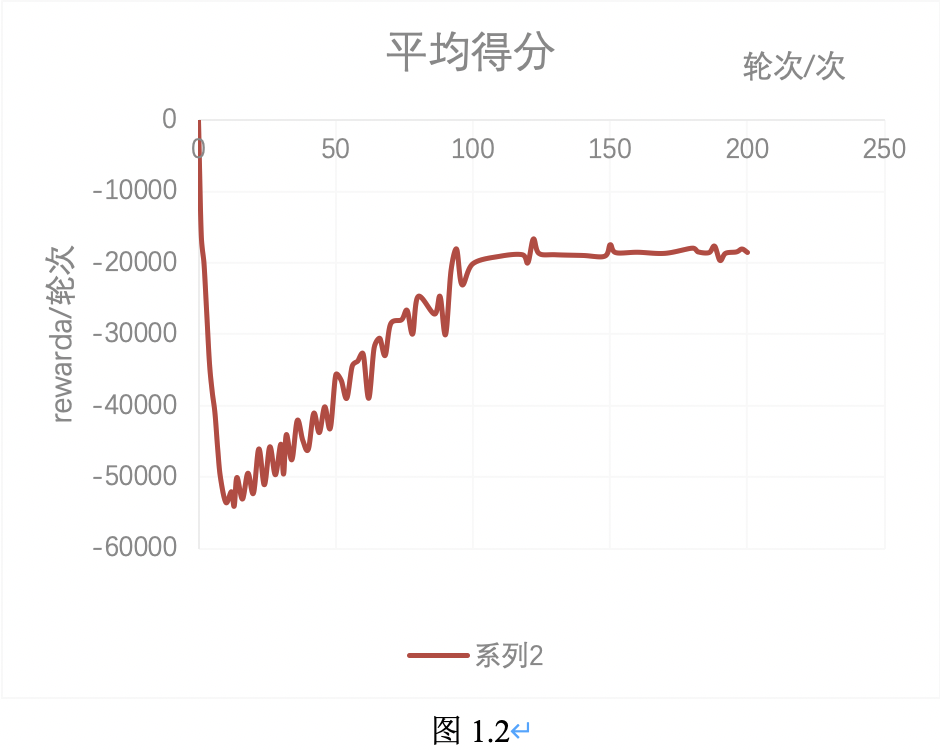
\includegraphics[height=.4\textheight]{pic/23.png}
        \end{figure}
    \end{minipage}
    
    \item 有没有可能得到比较平滑的曲线图呢?
    \item 我们可以取多次试验的平均结果,比如上面的图是一次试验过程中测试性能的曲线图,如果我们使用50个试验或100个试验,曲线图上每个点都为这50个或100个试验的平均结果,那么就可以得到一个比较平滑的曲线,但是这样可行性不高,因为强化学习本身就耗时较长,如果多次试验的话往往需要大量的计算时间。
    \item 此曲线只为归纳Q值变化,由于缺少平均得分进行对比,无法得出更多结论,在此不在赘述。

    
    \end{itemize}
    
\end{frame}





\begin{frame}{强化学习中性能的评价指标到底应该如何选择?}
    \begin{itemize}
    \tiny
    \item 平均Q值图像趋势与平均得分类似,但曲线相较平均得分光滑。
   

    
        \begin{minipage}{0.5\linewidth}
        \medskip
        %\hspace{2cm}
        \begin{figure}[h]
            \centering
            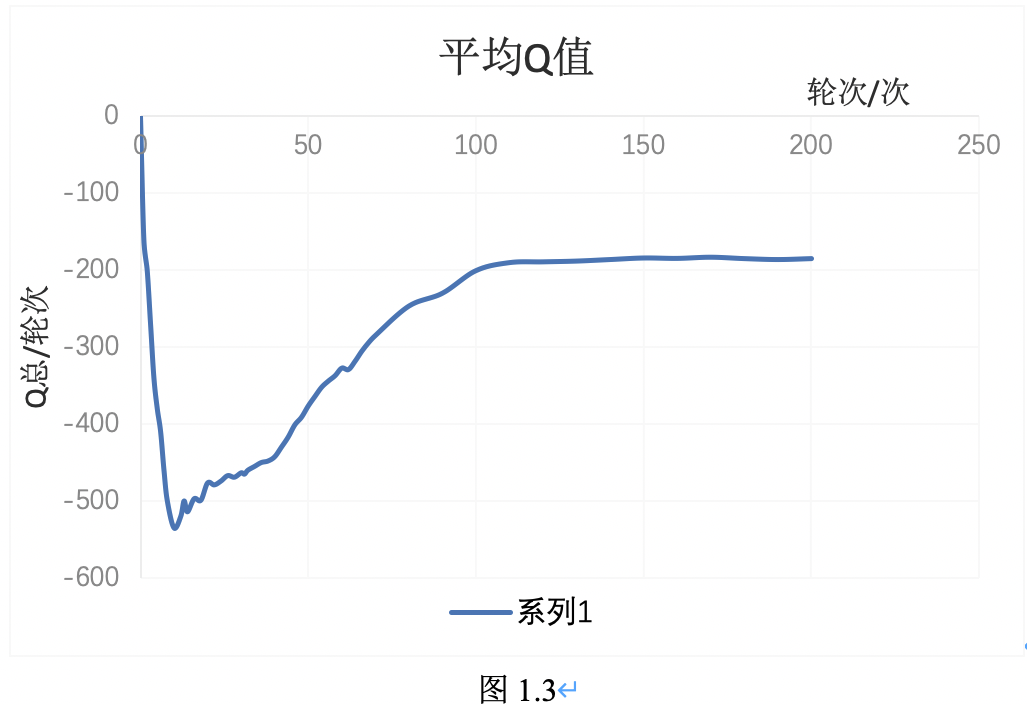
\includegraphics[height=.4\textheight]{pic/24.png}
        \end{figure}
    \end{minipage}
    
    \item 平滑性:可以看到使用平均得分法的评价方法(图1.2)不同轮次下对应的rewards随轮次数变化会具备较大的抖动性,相邻轮次对应的得分往往有很大差距,但是从整体来看平均得分法依然可以看到整体性能的变化趋势。平均Q值的方法(图1.3),可以看到不同轮次对应的Q值变化趋势比较平稳。

    \item 性能评价图所呈现的平稳性的差距是由什么所造成的,可以说评价Q值法比平均得分法好吗?
    \item 平滑性造成的原因:平均得分法每次进行性能评估时所执行的轮次下的状态动作序列都是不同的,而由于标准的训练方法会导致算法往往在某个时刻下对某些状态可以给出很好的决策,而对某些状态给出较差的决策。
    \item 但平均Q值法不能很好的刻画算法的实际性能,由于测评性能的状态动作对都是算法运行之前就已经固定好的,所以当算法运行到一定程度后对这些早已固定好的状态动作对的性能也就达到了稳定,虽然此时的平均Q值法获得的曲线图已经平稳但是却很难显示出当前算法的实际性能,因为此时算法的策略往往可能遇到一些之前难以遇到或者没有遇到过的状态,而平均Q值法难以对这些之前没有遇到过的状态进行测评。
    \item 因此,我们还是使用平均得分法作为算法性能的最终测评方法。

    
    \end{itemize}
    
\end{frame}




\section{参考文献}

\begin{frame}{参考文献}
    %\bibliography{ref}
    %\bibliographystyle{alpha}
    % 如果参考文献太多的话,可以像下面这样调整字体:
    %\tiny\bibliographystyle{alpha}
    %\nocite{*}
    [1] 基于不完全信息随机博弈与Q-learning的防御决策方法 - 张红旗 杨峻楠 张传富 - 《 通信学报 》 - 2018, 39(8)
    
    [2] 基于Q学习算法和BP神经网络的倒立摆控制-蒋国飞 吴沧浦-《 自动化学报 》-1998,24(5)
    
    [3] 基于Q学习算法和遗传算法的动态环境路径规划-于乃功 王琛 默凡凡 蔡建羡-《 北京工业大学学报 》-2017,43(7)
    
    [4]Bilibili网站《莫烦python》强化学习课程
    
    [5]CSDN Python-Tkinter图形化界面设计(详细教程 )—王张飞
\end{frame}



\begin{frame}
    \begin{center}
        {\Huge\calligra Thanks!}
    \end{center}
\end{frame}

\end{document}